%*****************************************************************************************
%*********************************** Second Chapter **************************************
%*****************************************************************************************

\newcommand{\unitDst}{\text{uDst}} % Destination in the unit range 0:1
\newcommand{\uDst}{\unitDst}       % Destination in the unit range 0:1
\newcommand{\intDst}{\text{iDst}}  % Destination in the integer range dstMin:dstMax
\newcommand{\iDst}{\intDst}        % Destination in the integer range dstMin:dstMax
\newcommand{\dstMax}{\text{dstMax}}      % Destination integer range maximum
\newcommand{\dstMin}{\text{dstMin}}      % Destination integer range mimimum
\newcommand{\dstRange}{\text{dstRange}}  % Destination integer range
\newcommand{\discreteDst}{\widetilde{\uDst}}   % Destination found using the discretized transformation matrix
\newcommand{\dDst}{\discreteDst}               % Destination found using the discretized transformation matrix
\newcommand{\delDst}{\delta\uDst}              % Error in the Destination found using the discretized transformation matrix

\newcommand{\unitT}{\text{uT}}             % Rotated values in the unit range 0:1
\newcommand{\uT}{\unitT}                   % Rotated values in the unit range 0:1
\newcommand{\intT}{\text{iT}}              % Rotated values in the integer range tMin:tMax
\newcommand{\iT}{\intT}                    % Rotated values in the integer range tMin:tMax
\newcommand{\tMax}{\text{tMax}}            % Rotated values integer range maximum
\newcommand{\tMin}{\text{tMin}}            % Rotated values integer range mimimum
\newcommand{\tRange}{\text{tRange}}        % Rotated values integer range
\newcommand{\discreteT}{\widetilde{\uT}}   % Rotated values found using the discretized transformation matrix
\newcommand{\dT}{\discreteT}               % Rotated values found using the discretized transformation matrix
\newcommand{\delT}{\delta\uT}              % Error in the Rotated values found using the discretized transformation matrix

\newcommand{\unitSrc}{\text{uSrc}}       % Source in the unit range 0:1
\newcommand{\uSrc}{\unitSrc}             % Source in the unit range 0:1
\newcommand{\intSrc}{\text{iSrc}}        % Source in the integer range srcMin:srcMax
\newcommand{\iSrc}{\intSrc}              % Source in the integer range srcMin:srcMax
\newcommand{\srcMax}{\text{srcMax}}      % Source integer range maximum
\newcommand{\srcMin}{\text{srcMin}}      % Source integer range mimimum
\newcommand{\srcRange}{\text{srcRange}}  % Source integer range

\newcommand{\unitX}{\text{uX}}       % Source in the unit range 0:1
\newcommand{\uX}{\unitX}             % Source in the unit range 0:1
\newcommand{\intX}{\text{iX}}        % Source in the integer range xMin:xMax
\newcommand{\iX}{\intX}              % Source in the integer range xMin:xMax
\newcommand{\xMax}{\text{xMax}}      % Source integer range maximum
\newcommand{\xMin}{\text{xMin}}      % Source integer range mimimum
\newcommand{\xRange}{\text{xRange}}  % Source integer range

\newcommand{\unitY}{\text{uY}}       % Destination in the unit range 0:1
\newcommand{\uY}{\unitY}             % Destination in the unit range 0:1
\newcommand{\intY}{\text{iY}}        % Destination in the integer range yMin:yMax
\newcommand{\iY}{\intY}              % Destination in the integer range yMin:yMax
\newcommand{\yMax}{\text{yMax}}      % Destination integer range maximum
\newcommand{\yMin}{\text{yMin}}      % Destination integer range mimimum
\newcommand{\yRange}{\text{yRange}}  % Destination integer range

\newcommand{\unitR}{\text{uR}}
\newcommand{\uR}{\unitR}
\newcommand{\intR}{\text{iR}}
\newcommand{\iR}{\intR}
\newcommand{\discreteR}{\widetilde{\uR}}
\newcommand{\dR}{\discreteR}
\newcommand{\delR}{\delta\uR}


\chapter{Color Spaces and Information Storage for Computer Vision Processing}

\ifpdf
    \graphicspath{{Chapter2/Figs/Raster/}{Chapter2/Figs/PDF/}{Chapter2/Figs/}}
\else
    \graphicspath{{Chapter2/Figs/Vector/}{Chapter2/Figs/}}
\fi


\section{Constructing a New Color Space}\label{sec:ConstructingANewColorSpace}

In order to construct a new color space, we need to consider the coordinate system of the new color space, the orientation of the new color space, and the fidelity of the discrete representation of the axes.

The first consideration is most easily decided; because there's little obvious advantage otherwise, we choose a Cartesean coordinate system as this allows for a straightforward transformation involving only rotation, translation and scaling. Because we're interested in the color information in the image, it's useful to design the color space so there is a luminosity axis. This choice determines two of three rotational degrees of freedom, as will be discussed below.

As for the discrete representation of the axes, it's desired that all the information captured pertaining to a hand should be preserved; all other information is irrelevant. However, here we'll consider only the effect of a rotation and scaling on the discrete representation.


\subsection{Camera RGB and Normalization for Discrete Range}\label{sec:CameraRGB}

Due to the hardware being locked down at the application level, we do not have access to the raw camera feed. We do, however, have access to the compressed, post-processing 8-bit RGB image data. The processing involves evening up the color channel senors' sensitivity by way of multiplying each channel by an appropriate correction factor. This is partly why cameras likely have a 10 or 12 bit/channel capture rate, but after accounting for differences in sensitivity, it only outputs in 8-bit color depth.

The three-color RGB channel sensors commonly found in CCD cameras are based on how the human eye perceives colors. But in physical reality, light is actually hitting the camera as a continuous spectrum. Since it's impossible to map an infinite set of Gaussians to it, we instead use some function which, for any frequency, will give the intensity of the light hitting the point at that frequency. This function is expanded in the basis set of three Gaussians with mean values centered on the RGB frequencies. This model is used in cameras because the main purpose of cameras --- until recent times --- has been to capture images for human viewing. And while the RGB Gaussian basis model is perfectly suited for capturing all the scene information which humans can perceive, it is not a complete representation.

Because we're searching for particular points in the real color space --- which, being a continuous function, is infinite dimensional --- there is a possibility in the future that larger multi-channel color spaces will be much more common, such as the 8-channel color spaces currently in development. Though most such cameras are primarily designed for post-production editing for still pictures and film (e.g. changing the lighting independent of the scene), as well as visual effects, the possibilities for computer vision are exciting. However, computer vision tasks are computationally intensive, and more often than not require operation in real time, so there is a natural inclination to shy away from large data sets in practical computer vision applications; many tasks are done in grayscale or single channel processing to expedite the process.

As such, there is a need to develop techniques which keep the relevant information while quickly and efficiently discarding the irrelevant information. This is true for the RGB space at the moment, and the aim of this first part of the work.

\subsection{iPhone Camera Characteristics} \label{sec:iPhoneCameraCharacteristics}

Unlike more general cameras, the iPhone's camera performs certain pre-processing tasks on the raw image before it reaches the AP layer. Typically, cameras have a specific white point value, which is the value corresponding to white. It isn't necessarily the corner of the RGB cube; finding this value is part of the camera calibration. It also determines the orientation of the luminosity axis, which passes through zero to the white point. This is why all pre-defined color space functions have an implicit white point correction. However, the iPhone's white point is always set to the corner of the RGB cube before the image reaches the AP layer. So, when developing an algorithm for the iPhone, white point correction is not necessary, while on other devices the algorithm may need to be adapted accordingly.

\begin{figure}[h!]
  \centering
    \includegraphics[width=0.80\textwidth]{Chapter2/Figs/lxy_general_white_point.eps}
    \caption{The white point for the general skin sample set described in Section~\ref{sec:SkinStatistics}.}  \label{fig:WhitePoint}
\end{figure}

While gathering skin statistics for the purposes of this project, the original approach involved taking photos of individual skin --- each with distinct color characteristics --- taken under different lighting conditions with a constant background using the iPhone camera. The background was included in order to obtain data on the edges of the skin. The background would be photographed, then again with each individual's hand over the same background. Afterward, the statistics would be collected and the background removed by negating the background statistics.

Surprisingly, this approached failed to work; the background reappeared (Figure~\ref{fig:BGFailure}).

\begin{figure}[h!]
  \centering
    \includegraphics[width=0.60\textwidth]{Chapter2/Figs/xy_bg_failed.eps}
    \caption{Initial attempt at removing background; unsuccessful.} \label{fig:BGFailure}
\end{figure}

The background statistics changed with the skin present in the photo. This is because the iPhone adjusts to images with very strong color characteristics. This is an undocumented feature of the iPhone processing. The only way to compensate for this unwelcome pre-processing is to photograph the background with a strongly contrasting object present, but one which is easily cropped out of the image before the background stats are collected. After collecting the statistics again, the result was much improved (Figure~\ref{fig:BGSuccess}).

\begin{figure}[h!]
  \centering
    \includegraphics[width=0.60\textwidth]{Chapter2/Figs/bg_cap.eps}
    \caption{The red marker cap contrasts with the green background.}  \label{fig:BGCap}
\end{figure}

\begin{figure}[h!]
  \centering
    \includegraphics[width=0.60\textwidth]{Chapter2/Figs/xy_bg_success.eps}
    \caption{Successful background removal.}  \label{fig:BGSuccess}
\end{figure}

In a real world context, it is relatively safe to presume that the scene will be chromatically complex enough that the color correction won't be detrimental to detection, and perhaps even beneficial under unusual lighting conditions. But for gathering statistics, it proved to be a massive pain.

\subsection{Rotation Matrix}\label{sec:RotationMatrix}
Any rotation about an axis can be represented by a matrix. Such rotations can be expressed as a 3x3 square matrix in a 3D space. Since they are generally invertible, they're guaranteed to be non-singular. For this application, we require rotation about three different axes, which can be expressed thus:


\begin{alignat}{1}
R_x(\theta) &= \begin{bmatrix}
1 & 0 & 0 \\
0 & \cos \theta &  -\sin \theta \\[3pt]
0 & \sin \theta  &  \cos \theta \\[3pt]
\end{bmatrix} \\[6pt]
R_y(\theta) &= \begin{bmatrix}
\cos \theta & 0 & \sin \theta \\[3pt]
0 & 1 & 0 \\[3pt]
-\sin \theta & 0 & \cos \theta \\
\end{bmatrix} \\[6pt]
R_z(\theta) &= \begin{bmatrix}
\cos \theta &  -\sin \theta & 0 \\[3pt]
\sin \theta & \cos \theta & 0\\[3pt]
0 & 0 & 1\\
\end{bmatrix}
\end{alignat}


It should be noted that the solutions are not unique; there are many ways in which to rotate an object from one position to another, or use a combination of different rotations to get to the same point, so they aren't necessarily unique, but this has no bearing on this project. So any rotation which orients the RGB color space such that one of the new axes lies along the luminosity direction is sufficient. To achieve this end using rotations about the RGB color space axes requires a rotation in only two of those axes.

A rotation which aligns the L axis along the luminosity direction is produced by a rotation of $\frac{\pi}4$ about the x axis, followed by a rotation of $\arctan{\frac{1}{\sqrt{2}}}$ about the y axis. This leaves one free rotational degree of freedom about the L axis. The resulting rotation matrix is given by:

\begin{equation}
R_{xyz}(\theta) =
\left(
\begin{array}{ccc}
 \frac{1}{\sqrt{3}} & \frac{1}{\sqrt{3}} & \frac{1}{\sqrt{3}} \\
 -\sqrt{\frac{2}{3}} \sin \left(\theta +\frac{\pi }{6}\right) & \sqrt{\frac{2}{3}} \cos (\theta ) & -\sqrt{\frac{2}{3}} \sin \left(\frac{\pi }{6}-\theta \right) \\
 -\sqrt{\frac{2}{3}} \cos \left(\theta +\frac{\pi }{6}\right) & -\sqrt{\frac{2}{3}} \sin (\theta ) & \sqrt{\frac{2}{3}} \cos \left(\frac{\pi }{6}-\theta \right) \\
\end{array}
\right)
\end{equation}


Where $\theta$ is the remaining rotational degree of freedom.

Using the standard rotation matrices, we get a luminosity axis from 0 to $\sqrt{3}$. However, the length of the two remaining axes are dependent on the value of $\theta$ used. This is a problem because, ultimately, we want the axes to fit in a range of an appropriate data type. It would be more useful to have a matrix which provided the specified rotation and scaled the axis to known lengths. In the case of the luminosity, this is straightforward; simply divide by $\sqrt{3}$. In the case of the other two axes, we need an explicit form for the lengths of the axis resulting from the rotation.

Because the absolute values of the axes in the color space have no meaning, we're only interested in the position along the axis relative to its start and end, equivalent to talking about the position in the axis relative to $0:1$, compared to about 0-255 in unsigned, 8-bit integers. The upside is that if we're rotating the cube about its corner, we're interested in the minimum and maximum values possible along the new axis direction, which will correspond to a corner of the RGB cube. With the L axis aligned along the luminosity direction, the range of the L axis is 0 to $\sqrt{3}$. The x and y axes are symmetrical, spanning a range centered on 0. The range of their values is dependent upon the remaining degree of freedom.

We need to know, in each of the axes, how far out each point is. Because we're effectively rotating a hexagon, whatever the answer is, we know the function is going to be periodic, repeating every $\frac{\pi}{3}$ radians, so we only have to solve it in the 0 to $\frac{\pi}{3}$ region and then generalize. First we take the cooordinates of the RGB cube and perform the rotation to find the values in the new color space.


\begin{multline}\label{eq:YabCube}
  R_{xyz}(\theta)\cdot\left(
\begin{array}{cccccccc}
 0 & 1 & 1 & 0 & 0 & 0 & 1 & 1 \\
 0 & 0 & 1 & 1 & 1 & 0 & 0 & 1 \\
 0 & 0 & 0 & 0 & 1 & 1 & 1 & 1 \\
\end{array}
\right) = \\
\resizebox{\textwidth}{!}{%
$\displaystyle
\left(
\begin{array}{cccccccc}
 0 & \frac{1}{\sqrt{3}} & \frac{2}{\sqrt{3}} & \frac{1}{\sqrt{3}} & \frac{2}{\sqrt{3}} & \frac{1}{\sqrt{3}} & \frac{2}{\sqrt{3}} & \sqrt{3} \\
 0 & -\sqrt{\frac{2}{3}} \sin \left(\theta +\frac{\pi }{6}\right) & \sqrt{\frac{2}{3}} \sin \left(\frac{\pi }{6}-\theta \right) & \sqrt{\frac{2}{3}} \cos (\theta ) & \sqrt{\frac{2}{3}} \sin \left(\theta +\frac{\pi }{6}\right) & -\sqrt{\frac{2}{3}} \sin \left(\frac{\pi }{6}-\theta \right) & -\sqrt{\frac{2}{3}} \cos (\theta ) & 0 \\
 0 & -\sqrt{\frac{2}{3}} \cos \left(\theta +\frac{\pi }{6}\right) & -\sqrt{\frac{2}{3}} \cos \left(\frac{\pi }{6}-\theta \right) & -\sqrt{\frac{2}{3}} \sin (\theta ) & \sqrt{\frac{2}{3}} \cos \left(\theta +\frac{\pi }{6}\right) & \sqrt{\frac{2}{3}} \cos \left(\frac{\pi }{6}-\theta \right) & \sqrt{\frac{2}{3}} \sin (\theta ) & 0 \\
\end{array}
\right)$}
\end{multline}


The extent of the new axis is found by taking the maximum and minimum values of each row i.e. the extreme corner positions relative to each new axis. An additional symmetry of the hexagonal projection of the RGB cube allows us to say that whatever functional form is taken by one of the $\theta$ dependant ranges the other can be found by a simple phase shift. So recognising that the minimum value is simply $-1$ times the maximum we have simplified the problem to solving

\begin{equation}\label{eq:AxisRangeMinMax}
 \max\left(\pm\frac{\sin (\theta )}{\sqrt{6}}\pm\frac{\cos (\theta )}{\sqrt{2}}, \pm\sqrt{\frac{2}{3}} \sin (\theta ) \right) \quad \text{Where} \quad 0\leq \theta \leq \frac{\pi}{3}
\end{equation}

A graphical representation of the problem can be seen in Figure~\ref{eq:YabCube}.

\begin{figure}[h!]
  \centering
    \includegraphics[width=\textwidth]{Chapter2/Figs/YABCubeEval.eps}
    \caption{Evaluation of the color space problem.}\label{fig:YABCubeEval}
\end{figure}

In the range 0 to $\frac{\pi}{3}$, both sin and cos are positive, therefore the axis ranges are given by the following:


\begin{tabular}{|c|c|c|}
  \hline
     & Min & Max \\ \hline
  X & \(0\) & \(\sqrt{3}\) \\
  Y & \(-\frac{\sin \left((\left(\theta -\frac{\pi }{6}\right) \bmod \frac{\pi }{3})\right)}{\sqrt{6}}-\frac{\cos \left((\left(\theta -\frac{\pi }{6}\right) \bmod \frac{\pi }{3})\right)}{\sqrt{2}}\) & \(\frac{\sin \left((\left(\theta -\frac{\pi }{6}\right) \bmod \frac{\pi }{3})\right)}{\sqrt{6}}+\frac{\cos \left((\left(\theta -\frac{\pi }{6}\right) \bmod \frac{\pi }{3})\right)}{\sqrt{2}}\) \\
  Z & \(-\frac{\sin \left((\theta  \bmod \frac{\pi }{3})\right)}{\sqrt{6}}-\frac{\cos \left((\theta  \bmod \frac{\pi }{3})\right)}{\sqrt{2}} \) & \(\frac{\sin \left((\theta  \bmod \frac{\pi }{3})\right)}{\sqrt{6}}+\frac{\cos \left((\theta  \bmod \frac{\pi }{3})\right)}{\sqrt{2}}\) \\
  \hline
\end{tabular}

\begin{tabular}{|c|c|c|}
  \hline
  % after \\: \hline or \cline{col1-col2} \cline{col3-col4} ...
    & Min & Max \\ \hline
  X & \(0\) & \(\sqrt{3}\) \\
  Y & \(- \sqrt{\frac{2}{3}} \cos \left(\frac{\pi }{6}-(\left(\theta -\frac{\pi }{6}\right) \bmod \frac{\pi }{3})\right) \)&\( \sqrt{\frac{2}{3}} \cos \left(\frac{\pi }{6}-(\left(\theta -\frac{\pi }{6}\right) \bmod \frac{\pi }{3})\right) \)\\
  Z & \(-\sqrt{\frac{2}{3}} \cos \left(\frac{\pi }{6}-(\theta  \bmod \frac{\pi }{3})\right) \)&\( \sqrt{\frac{2}{3}} \cos \left(\frac{\pi }{6}-(\theta  \bmod \frac{\pi }{3})\right) \)\\
  \hline
\end{tabular}

The lengths of the axis after rotation are given by:
\begin{equation}\label{eq:L}
\mathbf{L}(\theta) = \left(
\begin{array}{c}
\sqrt{3} \\
 \sqrt{\frac{2}{3}} \sin \left(\widetilde{\vartheta}\right) + \sqrt{2} \cos \left(\widetilde{\vartheta}\right) \\  
\sqrt{\frac{2}{3}} \sin \left(\widetilde{\theta}\right) + \sqrt{2} \cos \left(\widetilde{\theta}\right) 
\end{array}
\right)
\quad \text{where}  \quad 
\begin{array}{c}
\widetilde{\theta} = \theta  \bmod \frac{\pi }{3} \\ 
\widetilde{\vartheta} = \left(\theta - \frac{\pi }{6}\right) \bmod \frac{\pi }{3}
\end{array}
\end{equation}

It is convenient to produce a transformation which will result in axes of known length. Because the rotation cannot include a translation, we desire a transformation matrix which will result in the ranges $0:1$, -$\frac{1}2$ to $\frac{1}2$, and -$\frac{1}2$ to $\frac{1}2$. Such a transformation is easily obtained by multiplying the rotation matrix by a diagonal matrix with the reciprocal of the maximums found above placed along the diagonal. This will scale each axis to a unit length.

The normalized 'rotation' matrix is given by:


\begin{equation}\label{eq:NormRxyz2}
 \overline{R}_{xyz}(\theta) =
\left(
\begin{array}{c}
 \frac{1}{\sqrt{3}}  \\
 \frac{1}{L_2(\theta)} \\
 \frac{1}{L_3(\theta) }  \\
\end{array}
\right)
\bigotimes
R_{xyz}(\theta)
\end{equation}

\begin{gather*}
  \widetilde{\theta} = \theta  \bmod \frac{\pi }{3} \\
\widetilde{\vartheta} = \left(\theta +\frac{\pi }{6}\right) \bmod \frac{\pi }{3}
\end{gather*}
\begin{equation}\label{eq:NormRxyz}
\overline{R}_{xyz}(\theta) =
\left(
\begin{array}{ccc}
 \frac{1}{3} & \frac{1}{3} & \frac{1}{3} \\
 -\frac{\sqrt{3} \cos (\theta )+3 \sin (\theta )}{3 \cos \left(\widetilde{\vartheta}\right)+\sqrt{3} \sin \left(\widetilde{\vartheta}\right)} & \frac{2 \sqrt{3} \cos (\theta )}{3 \cos \left(\widetilde{\vartheta}\right)+\sqrt{3} \sin \left(\widetilde{\vartheta}\right)} & \frac{3 \sin (\theta )-\sqrt{3} \cos (\theta )}{3 \cos \left(\widetilde{\vartheta}\right)+\sqrt{3} \sin \left(\widetilde{\vartheta}\right)} \\
 \frac{\sqrt{3} \sin (\theta )-3 \cos (\theta )}{3 \cos \left(\widetilde{\theta}\right)+\sqrt{3} \sin \left(\widetilde{\theta}\right)} & -\frac{2 \sqrt{3} \sin (\theta )}{3 \cos \left(\widetilde{\theta}\right)+\sqrt{3} \sin \left(\widetilde{\theta}\right)} & \frac{3 \cos (\theta )+\sqrt{3} \sin (\theta )}{3 \cos \left(\widetilde{\theta}\right)+\sqrt{3} \sin \left(\widetilde{\theta}\right)} \\
\end{array}
\right)
\end{equation}

\section{Skin Statistics}\label{sec:SkinStatistics}

In order to identify the range of values for the skin space, a large number of skin samples were taken from photographs from the Humane project by Angelica Dass, an ongoing "chromatic inventory" art project which aims to compile every possible human skin color, categorized by the PANTONE guide color classification system~\cite{Dass2012}. The skin colors catalogued thus far are independent of race or ethnicity, so the samples are representative of human skin tones in general.

The image set consists of approximately 200 skin samples --- each of which shows only skin --- which are placed in a single directory in the file system. In accordance to our assumption that luminosity is not a significant factor in our skin model, we then perform the transformation initially with the value of $\theta$ equal to 0. The Matlab code collects frequency data for the rotated color space, incrementing the counts of a three-dimensional array of bins which span the color space. Viewing the frequency data along each of the three axes reveals that the skin image characteristics are spread widely in luminosity, but are quite confined in hue and saturation as illustrated in Figure~\ref{fig:InitBins}.


\begin{figure}[h!]
  \centering
    \includegraphics[width=\textwidth]{Chapter2/Figs/InitialBins.eps}
    \caption{Initial set of bins.}  \label{fig:InitBins}
\end{figure}


Aside from differing lighting, this is consistent with the notion that skin has a distinct pigmentation and justifies our attempt to find an appropriate color space disregarding luminosity. In doing so, the distribution of the skin color characteristics neatly fit into a 2-dimensional Gaussian distribution. The Matlab code produces a fit with a 2-dimensional Gaussian distribution and provides an angle relative to the orientation of the Gaussian fit to the skin sample distribution in the current color space.

Given that we are free to choose the orientation of the color space about the luminosity axis, the Matlab code allows us to find an orientation $\theta$ of the color space about the luminosity axis in which the distribution can be expressed as a product of 1-dimensional Gaussians along the axes. The final resulting distribution is presented in Figure~\ref{fig:DistributionAndGaussianFit}.


\begin{figure}[h!]
  \centering
    \includegraphics[width=\textwidth]{Chapter2/Figs/crosshairFigureFinal.eps}
    \caption{Distribution and Gaussian fit to the chromatic pixel values in the new color space.}  \label{fig:DistributionAndGaussianFit}
\end{figure}


For numerical reasons, the value for $\theta$ was found iteratively by performing the color space transformation and the statistical fit until the value for $\theta$ converged. (See Figure~\ref{fig:ConvergenceTheta}.)


\section{Implementation of Skin Color Space Statistics in Matlab}\label{sec:SkinColorSpaceStatsMatlab}

A naive approach is to take a directory of images and process them using our color space transformation with the free angle $\theta$, processing them into three-dimensional pixel value bins. It was discovered that the region of interest is relatively small in this 3D space, so it was made possible the use of a bin of width greater than 1 lumio-chromatic value. However, it is quickly found that the region of interest is so small that using a more encompassing lumio-chromatic bin is actually detrimental to the numerics involved in finding and appropriate Gaussian fit, so a lumio-chromatic bin of width 1 is used.

Because the region is so small, when the transformation is applied, we must also retain all the information therein. Initially, we did not know this; our transformed images were represented as the same data type as the original. But because the transformed information is a less efficient representation of the original information, a significant amount of that information is lost.

\begin{figure}[h!]
  \centering
    \includegraphics[width=\textwidth]{Chapter2/Figs/ConvergenceOfSkinSpaceFinal.eps}
    \caption{Convergence of color space orientation $\theta$.}  \label{fig:ConvergenceTheta}
\end{figure}

A better approach would be to iterate over the free angle $\theta$ of the Gaussian fit of the two-dimensional bin, which was found by collapsing the 3D bins along the luminosity axis, until convergence; at best, convergence was achieved after 3 iterations. Unfortunately, this approach --- though conceptually straightforward --- is very wasteful; all of the necessary information can be found in the RGB bin statistics.

Given that we are unable to apply this process in a reasonably efficient manner to individuals and general samples, if this project is to be finished sometime this century, a more nuanced approach is necessary.

\subsection{Transformation with Zero Angle}\label{sec:TransWithZeroAngle}

The more interpretable statistics for this project is a set of bins which contains all the information in the RGB bins, but is oriented such that there is a luminosity axis and two chromatic axes. Although the rotation matrices aren't unique, a set can be chosen and an angle $\theta$ determined in the chromatic space to be zero.

\begin{figure}[h!]
  \centering
    \includegraphics[width=0.49\textwidth]{Chapter2/Figs/xy_Polygon.eps}
    \caption{The projection along the L axis showing the chromatic space with a free rotational angle of 0.}  \label{fig:xyPolygon}
\end{figure}



\subsection{Removing Zeroes}\label{sec:RemovingZeroes}

The obvious idea is to find all the non-zero bins and fit an interpolating function between them. This will effectively remove the empty bin artifacts within the density-packed region which is the distribution we're interested in. However, the empty bins outside the main distribution are not artifacts and are genuinely empty bins, so removing all the empty bins and then fitting the function joins together any outlying points or secondary distributions corresponding to regions such as the background. We therefore desire a method which will allow us to keep all the non-empty bins and the empty bins outside the main distribution, i.e. all the genuinely empty bins. To achieve this, we designed a Matlab routine which essentially paints a region around each non-zero point, marking it as part of the main distribution. It then takes all the unmarked regions and includes all the empty bins in those regions. So, the set of points which is all the non-empty bins and all the empty bins in the unmarked regions satisfies the requirement, and a simple interpolating function can easily be fitted to those points.

%<flow chart, maybe? Or maybe at the end; we'll see.>

\subsection{White-Out and Black-Out}\label{sec:WhiteOutBlackOut}

Naively collapsing the bins along the luminosity axis artificially skews the chromatic distribution along the axis which passed through the luminosity axis; this is easily explained due to white-out and black-out. As luminosity increases or decreases, it will eventually hit the edge of the cube. Having reached its numerical limit, the luminosity slides toward the corner of the cube, resulting in a white or black value.

To accommodate this, we collapse the bins excluding the bins which are clearly suffering from white-out and black-out. This could be done mathematically by taking the bin of the distribution which is furthest from the luminosity axis, and then finding the intersection with the RGB cube when this chromatic value is at its limits, just before it reaches the edge of the cube where it suffers from white-out or black-out. But it's a simple matter to look at the three projections of the 3D Lxy bins and manually determine the limits for the valid region.

%<Insert white-out/black-out bins here>

\subsection{Removing the Background Distribution}\label{sec:RemovingBGDistribution}

Having removed the empty bin artifacts and compensated for white-out/black-out effects, the final step is to remove the bin counts of the bins which are associated with the background, thereby leaving a distribution which corresponds to chromatic skin values and which is artifact- and systematic-error-free. With the chromatic bins processed as they have been so far, it is clear that there is a distinct distribution for the skin and a distinct distribution for the background. However, a distribution for the background was produced earlier, compensating for the iPhone's pre-AP-layer processing. Background removal is automated using a Matlab function which will negate the bins from one sample set using the distribution found for a second sample set.

%<Graph showing the overlap of the background and a skin background sample set; briefly describe what that shows.>

\subsection{Results}\label{sec:Results}

We're trying to develop a skin model from the Humane project, which provides a set which spans all the different skin tones. Although these images are not captured using the iPhone camera and thus suffer from a white point which does not correspond with the iPhone's white point (at least at the AP layer), it does provide a sufficient statistical basis to determine a color space region which is spanned by human skin. However, because of the iPhone camera's characteristics after pre-processing and the fact that the application needs to respond to an individual's skin, the investigation of skin tone characteristics for individuals is necessary.

To that effect, we selected three individuals with different skin tones; ordering by pigmentation from dark to light, we will henceforth refer to these as subjects F, N and J. Statistics were collected for the three subjects using the procedure outlined previously in this section. A two-dimensional Gaussian was fitted to the distribution for each individual.

\begin{figure}[h!]
  \centering
    \includegraphics[width=0.49\textwidth]{Chapter2/Figs/FHands_XY_fBin.eps}
    \includegraphics[width=0.49\textwidth]{Chapter2/Figs/FHands_XY_gFit.eps}
    \includegraphics[width=0.49\textwidth]{Chapter2/Figs/NHands_XY_fBin.eps}
    \includegraphics[width=0.49\textwidth]{Chapter2/Figs/NHands_XY_gFit.eps}
    \includegraphics[width=0.49\textwidth]{Chapter2/Figs/JHands_XY_fBin.eps}
    \includegraphics[width=0.49\textwidth]{Chapter2/Figs/JHands_XY_gFit.eps}
    \caption{The xy bins after processing and the Gaussian fit.}  \label{fig:FBinAndGFit}
\end{figure}

The individual statistics are as follows:
\newline

\begin{tabular}{|c|c|c|c|c|c|c|}
\hline
& \multicolumn{2}{|c|}{Mean ($\mu$)} & \multicolumn{2}{|c|}{Standard Deviation ($\sigma$)} & \multicolumn{2}{|c|}{Angle ($\theta$)} \\\hline
& X & Y & X & Y & Major Axis & Minor Axis \\\hline
F & 0.4249 & 0.3335 & 0.0081 & 0.0251 & -0.7724 & 0.7984 \\\hline
N & 0.4281 & 0.3443 & 0.0080 & 0.0195 & -0.5549 & 0.5969 \\\hline
J & 0.4022 & 0.3302 & 0.0119 & 0.0253 & -0.8954 & 0.6754 \\\hline
\end{tabular}
\newline
\vspace{0.5 cm}
\newline
The statistics for the general sample set are as follows:
\newline

\begin{tabular}{|c|c|c|c|c|c|c|}
\hline
& \multicolumn{2}{|c|}{Mean ($\mu$)} & \multicolumn{2}{|c|}{Standard Deviation ($\sigma$)} & \multicolumn{2}{|c|}{Angle ($\theta$)} \\\hline
& X & Y & X & Y & Major Axis & Minor Axis \\\hline
General & 0.4820 & 0.4253 & 0.0072 & 0.0108 & -0.1174 & 1.4534 \\\hline
\end{tabular}



\section{Preservation of Color Information}\label{sec:PreservationOfColorInformation}

The goal of the algorithm is to preserve all the information captured by the camera which relates to skin whilst discarding as much of the irrelevant information as possible. Given that edges and features often present as shadows and highlights, all the information captured in terms of luminosity will be regarded as relevant information, at least as far as the manipulation of individual pixel values is concerned. Considering the chromatic information, the importance of the pixel value will be directly determined by the Gaussian distribution found previously.

Knowing the range of values produced by the rotation allows us to scale the transformation to fit into the range of destination data type. If we have RGB pixel values in a given machine data type, the amount of information contained in each of those channels is equal to the number of values accessible in that data type. For example: for 8-bit, unsigned integers, there are 256 possible values. After a rotation, we are interested in the amount of information which lies along the new axes. This is found simply by multiplying the range of the source data type by the length of the new axes found for the unit cube. To preserve all the information captured, we would therefore have to use a larger data type to store the new values. We are, however, only interested in a small region in the chromatic space, at least. The question is, then, how to preserve the relevant information in a way consistent with the significance indicated by the Gaussian distribution found previously.





\begin{figure}[h!]
  \centering
    \includegraphics[width=\textwidth]{Chapter2/Figs/unitGraph.eps}
    \caption{Unit graph.}  \label{fig:UnitGraph}
\end{figure}


None of the rotated axes have lengths less than 1 for the unit RGB cube. For this reason we've written redistribution functions which perform any necessary type conversion whilst preserving the information in a controlled way; we can keep the information where it's needed and discard it where it's irrelevant. So although this is strictly beyond the normal meaning of a color space conversion, it is addressing a connected issue and belongs in the conversion. In terms of optimisation, it is also the most efficient place in the code in which to perform this adjustment, allowing us to --- for the sake of example --- discard the details of the colors of a duck's feathers whilst keeping the hues and tones of human skin.

We can use a function to redistribute the information contained on the longer axis onto the shorter axis, which can be expressed in the discrete representation of that axis necessitated by internal integer data types. There are three ways in which to implement the redistribution functions:

\subsection{Partition}\label{sec:Partition}

The most straightforward redistribution method is to simply preserve the information in a 1-to-1 fashion within a region. The region can be defined in terms of the skin color distribution Gaussian by specifying a significance level in terms of the variance or the standard deviation.

\subsection{Linear}\label{sec:Linear}

A slightly more sophisticated method is to use a linear redistribution. A linear distribution is equivalent to partitioning given a unit gradient. However, a linear redistribution function allows for the possibility of data compression. So then, in the case where the region of interest contains more information than can be expressed in the destination data type, a linear distribution function allows an even compression of the information from source to destination. ~\cite{Lee2002}

\subsection{ERF (Gaussian Error Function)}\label{sec:ERF}

The integral of the cumulative Gaussian (i.e. Error Function) allows the redistribution of the information on the axis in a way which selectively preserves the information about a point on the axis (i.e. the mean of the Gaussian), and then progressively discard the information as it falls into the tails of the Gaussian. So, it provides a non-linear distribution of the information. The Gaussian can be seen as describing our interest in the information contained along the axis, so it's logical to use the error function to redistribute the information. The disadvantage of this is simply the computational effort involved in generating the error function.

The error function distribution is mathematically correct, being directly related to the Gaussian fit. Computationally, there are two considerations: the numerical representation, and performance. The discrete representation of the numerics means that --- for a significant number of possible distributions --- distributing using the error function has little to no advantage (or indeed difference) from using a linear distribution.

Considering the preservation of information captured, mappings with a gradient greater than 1 are undesirable because they preserve all the information whilst being informatically wasteful in that there are functionally inaccessible discrete values in the destination range. Our stated aim is to preserve the information in the image pertaining to human skin; unevenly distributing this information across a discrete data type is not only wasteful in terms of memory, but also of processing resources because subsequent processing routines will treat the data as if it has a higher fidelity than it actually does.

To construct a distribution function, we first need to describe the relationship of the error function to the Gaussian fit, and then produce a function with the appropriate range and domain. For a Gaussian fit with an amplitude A, a mean of $\mu$, and a standard deviation of $\sigma$, where $\mu$ and x lie in a source range $\xRange$ from $\xMin$ to $\xMax$. The cumulative distribution is found by integrating from $\xMin$ to the point x, as can be seen in (\ref{eq:ErfDefinition}):

\begin{equation}\label{eq:ErfDefinition}
  \int _{\xMin}^{\text{x}} A \frac{e^{-\frac{(t-\mu )^2}{2 \sigma ^2}}}{\sqrt{2 \pi } \sigma }dt=\frac{1}{2} A \left(\text{erf}\left(\frac{\text{x}-\mu }{\sqrt{2} \sigma }\right)-\text{erf}\left(\frac{\xMin-\mu }{\sqrt{2} \sigma }\right)\right)
\end{equation}

The Gaussian distribution and the cumulative distribution are shown in Figure~\ref{fig:ErrorFunctionGraph} for some values chosen for illustrative purposes. All that is required now is to fix the range $\yMin$ to $\yMax$ for the domain $\xMin$ to $\xMax$.

\begin{figure}[h!]
  \caption{Error function.}  \label{fig:ErrorFunctionGraph}
  \centering
    \includegraphics[width=\textwidth]{Chapter2/Figs/errorFunction.eps}
\end{figure}

First, we determine the maximum value taken in the domain. This is simply found by evaluating the function at $\xMax$. It should be noted that --- if the Gaussian distribution is well-contained in the source domain --- the maximum value should be equal to the amplitude. For the sake of simplicity, we'll ignore the amplitude of the fitted Gaussian found previously as it is not relevant to the design of the redistribution function. So, to fix the range of the distribution function, we first scale to the range $0:1$ by simply dividing through by the maximum value, and then re-scale to the destination range $\yRange = \yMax - \yMin$ and shift by $\yMin$.

\begin{equation}\label{eq:disFunction}
  dis(x) = \frac{(\yRange) \left(\text{erf}\left(\frac{x-\mu }{\sqrt{2} \sigma }\right)-\text{erf}\left(\frac{\xMin-\mu }{\sqrt{2} \sigma }\right)\right)}{\text{erf}\left(\frac{\xMax-\mu }{\sqrt{2} \sigma }\right)-\text{erf}\left(\frac{\xMin-\mu }{\sqrt{2} \sigma }\right)}+\yMin
\end{equation}

Mathematically, this distribution function~(\ref{eq:disFunction}) achieves all the stated objectives. However, on a device we are dealing with discrete numerics and limited processing power, so further analysis is required. Where we're using a discrete domain and range, the distribution is usefully divided into three characteristic behaviors:  where it is constant, where it preserves all the information, and where it selectively preserves information. Looking at the distribution, this divides the source domain into five regions: two where it is effectively constant, two where it is selective, and one region around the mean where it preserves all the information. In order to design an efficient algorithm, it is useful to identify the boundaries of these five regions.

First, we need to identify where the distribution is effectively constant. This can be found by solving the following equation in the region and domain $0 \le x \le 1$ and then generalized to the specific discrete numerics:

\begin{equation}\label{eq:0to1}
 \frac{\text{erf}\left(\frac{\mu }{\sqrt{2} \sigma }\right)+\text{erf}\left(\frac{x-\mu }{\sqrt{2} \sigma }\right)}{\text{erf}\left(\frac{\mu }{\sqrt{2} \sigma }\right)-\text{erf}\left(\frac{\mu -1}{\sqrt{2} \sigma }\right)}=\text{dL} \quad \text{where} \quad \text{dL} = \left\{ \frac{1}{\yRange}, 1 - \frac{1}{\yRange} \right\}
\end{equation}


The solution is found for the source domain in the range $0:1$ as:


\begin{equation}\label{eq:LowHigh}
 x = \sqrt{2} \sigma  \text{erf}^{-1}\left((\text{dL}-1) \text{erf}\left(\frac{\mu }{\sqrt{2} \sigma }\right)-\text{dL} \; \text{erf}\left(\frac{\mu -1}{\sqrt{2} \sigma }\right)\right)+\mu
\end{equation}

To find the region where all the information in the source domain is preserved, we differentiate the distribution and solve for where the gradient is equal to the destination range over the source range. This corresponds to the point at which a unit change in the source produces a unit change in the destination range:

\begin{equation}\label{eq:Boundaries}
\frac{\sqrt{\frac{2}{\pi }} e^{-\frac{(x-\mu )^2}{2 \sigma ^2}}}{\sigma  \left(\text{erf}\left(\frac{\mu }{\sqrt{2} \sigma }\right)-\text{erf}\left(\frac{\mu -1}{\sqrt{2} \sigma }\right)\right)}=\frac{\yRange}{\xRange}
\end{equation}

Rearranging for $x$, we find:

\begin{equation}\label{eq:PreservedRegion}
 x=\mu \pm \sigma  \sqrt{-2 \log \left(\sigma  \left(\text{erf}\left(\frac{\mu }{\sqrt{2} \sigma }\right)-\text{erf}\left(\frac{\mu -1}{\sqrt{2} \sigma }\right)\right)\right)+2 \log \left(\frac{\xRange}{\yRange}\right)+\log \left(\frac{2}{\pi }\right)}
\end{equation}

We now have equations which gives us the four points in the source domain which mark the boundaries of the five characteristic regions. The equations are valid in the unit source domain $0:1$. It is a simple matter to scale and shift these values to give the points in a more general source domain.


\begin{equation}
\begin{aligned}
\Sigma^- &= \text{erf}\left(\frac{\mu -1}{\sqrt{2} \sigma }\right) &
 \Sigma^+ &= \text{erf}\left(\frac{\mu }{\sqrt{2} \sigma }\right) &
  \text{dL} &= \frac{1}{\yRange}
\end{aligned}
\end{equation}

\begin{equation}\label{eq:PreservedRegionGen}
\begin{aligned}
\Lambda^-(\mu,\sigma) &= \xMin + \xRange\left( \mu - \sigma  \sqrt{-2 \log \left(\sigma  \left(\Sigma^+-\Sigma^-\right)\right)+2 \log \left(\frac{\xRange}{\yRange}\right)+\log \left(\frac{2}{\pi }\right)}\right) \\
\Lambda^+(\mu,\sigma) &= \xMin + \xRange \left(\mu + \sigma  \sqrt{-2 \log \left(\sigma  \left(\Sigma^+-\Sigma^-\right)\right)+2 \log \left(\frac{\xRange}{\yRange}\right)+\log \left(\frac{2}{\pi }\right)}\right)
\end{aligned}
\end{equation}

\begin{equation}\label{eq:LowHighGen}
\begin{aligned}
\lambda^+(\mu,\sigma)  &=  \xMin + \xRange \left( \sigma \sqrt{2}  \text{erf}^{-1}\left((\text{dL}-1) \Sigma^- -\text{dL} \; \Sigma^+ \right)+\mu \right) \\
\lambda^-(\mu,\sigma)  &=  \xMin + \xRange \left( \sigma \sqrt{2} \text{erf}^{-1}\left((\text{dL}-1) \Sigma^+-\text{dL} \; \Sigma^-\right)+\mu \right)
\end{aligned}
\end{equation}



\begin{figure}[h!]
  \centering
    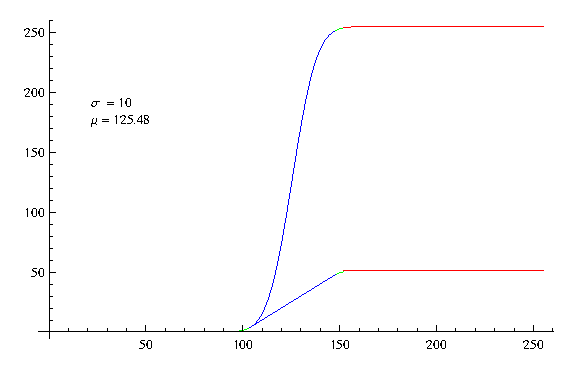
\includegraphics[width=0.49\textwidth]{Chapter2/Figs/partitionSmooth2.eps}
    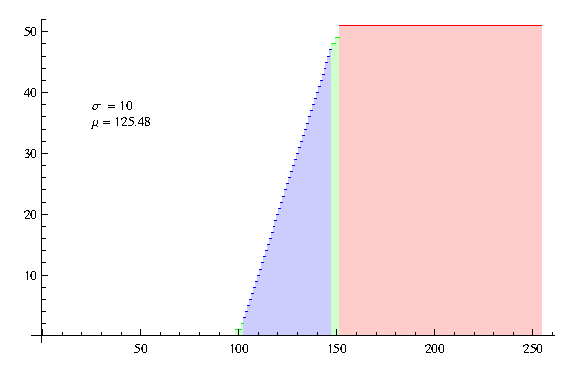
\includegraphics[width=0.49\textwidth]{Chapter2/Figs/partitionColor2.eps}
    \caption{Linear partition approximation.}  \label{fig:Partition}
\end{figure}

\begin{figure}[h!]
  \centering
    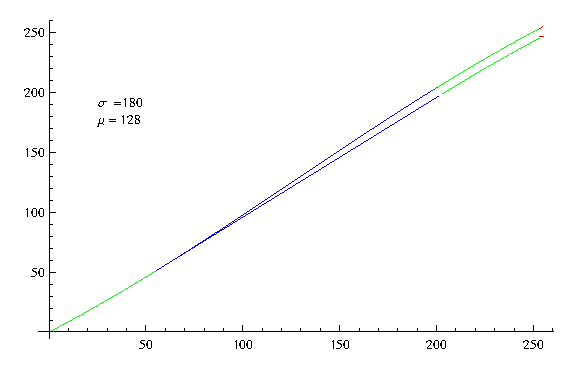
\includegraphics[width=0.49\textwidth]{Chapter2/Figs/linearSmooth2.eps}
    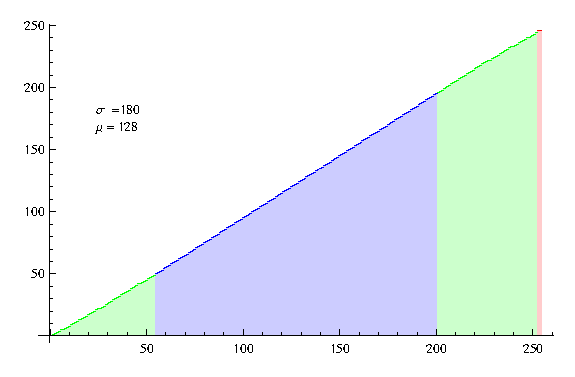
\includegraphics[width=0.49\textwidth]{Chapter2/Figs/linearColor2.eps}
    \caption{Linear approximation.}  \label{fig:Linear}
\end{figure}

\begin{figure}[h!]
  \centering
    \includegraphics[width=0.49\textwidth]{Chapter2/Figs/ERFSmooth2.eps}
    \includegraphics[width=0.49\textwidth]{Chapter2/Figs/ERFColor2.eps}
    \caption{Error Function distribution.}  \label{fig:ERF}
\end{figure}

There is one final value of interest to the development of the algorithm, which is the gradient at the mean. The reason this is of interest is because we're trying to compress the relevant data as much as possible. If the destination region is small (i.e. the destination machine type is smaller than the source type), then the gradient at the mean allows us to assess the fidelity required of the source type. If it weren't for the fact that the source is the result of a rotation transformation, then there would be little purpose in assessing this value. However, it is entirely possible that the lengthening of the axes resulting from the rotation is insignificant for the desired destination type; there's no point preserving information during the rotation which is then discarded by the redistribution. The gradient is given by

\begin{equation}\label{eq:gradient}
\Delta(\mu,\sigma) = \frac{\yRange}{\xRange}  \frac{ \sqrt{2} }{ \sigma \sqrt{\pi }  \left(\Sigma^+-\Sigma^-\right)}
\end{equation}

The required fidelity in the source domain can be found using $ \Delta$ in the sense that the correspondence between one information step in the source must produce a step of $\Delta$ in the destination type. For the algorithm evaluating the maximum gradient $\Delta$ allows us to be sure that  $\Lambda$ exists if $\Delta >1$ or tells us that the x axis can be shortened if  $\Delta < 1$. In the algorithm $\Delta$ is used to find an appropreate working data type for the rotated colorspace and to define the axis scaling for the rotation matrix.

\section{The Skin Color Space Algorithm}

Now that all of the values necessary to preserve the skin information have been obtained, we can use them to build a color space transformation algorithm which can make intelligent decisions about the numerical precision for the intermediate and final variables, as well as determining the most efficient transformation methods. The algorithm described herein will take values of $\theta$, the rotation about the luminosity axis, the standard deviations and mean values for the two chromatic axes, and will automatically decide upon the necessary intermediate working data types and the most efficient redistribution methods.

Previously, we found the lengths of the new axes after the rotational transformation. If we were to keep the same data type for the color space as is used for the RGB values, then the axes would have to be rescaled with the accompanying loss of information. Given that we have values which allow us to assess where all the relevant information lies, a more sophisticated approach is possible. For a chromatic axis --- which, after rotation, has a length $L(\theta)$ --- we can determine the positions on that axis at which the information is considered irrelevant using Equation~(\ref{eq:LowHigh}) and the positions where the information is all considered relavant. If the gradient \ref{eq:gradient} is less than 1, then the distribution looses information at all points on the axis and the axis can be shortened without loss of relavent information. The only further consideration is to ensure that the values outside that range are prevented from causing errors associated with overflow. To exclude this possibility, a conditional statement can be used which checks the bounds as stated, assigning an appropriate value as necessary. The alternative is to use an intermediate value with a higher bit depth, and then to recast into the destination data type in such a way that overflow and underflow are handled appropriately. The OpenCV library provides a casting method --- "saturateCast" --- which serves this purpose.

We need to consider the requested compression of information alongside the spread of information caused by the rotation, and the desired focus on the specific region of interest dictated by the statistics. Each axis in the color space is to be represented by a discrete set of numbers. The size of these sets dictates the discretization of the axis, and the ratios between them indicates the spread or compression of the information they contain. We assume that the RGB axes are each discretized to the same extent, each containing $\srcRange$ values. After the application of the un-normalized rotational transformation, the axes contain differing numbers of values given by $\tRange_1 =\srcRange \sqrt{3} $, $\tRange_2 = \srcRange L_2(\theta) $  and $\tRange_3 = \srcRange L_3(\theta)$. These axis lengths preserve all the information contained in the source colorspace and so are the maximum length which the axis should take. The minumum length the axis may take is where the information is lost evenly throuought the axis and corresponds to an axis length equal to the destination axis length $\tRange = \dstRange$. 

\begin{align}\label{eq:L}
L_1 &= \sqrt{3} \\
L_2(\theta)  &= \sqrt{\frac{2}{3}} \sin \left(\widetilde{\vartheta}\right) + \sqrt{2} \cos \left(\widetilde{\vartheta}\right)  & where & & \widetilde{\theta} = \theta  \bmod \frac{\pi }{3} \\
L_3(\theta)  &= \sqrt{\frac{2}{3}} \sin \left(\widetilde{\theta}\right) + \sqrt{2} \cos \left(\widetilde{\theta}\right) & & & \widetilde{\vartheta} = \left(\theta - \frac{\pi }{6}\right) \bmod \frac{\pi }{3}
\end{align}

The destination color space is designed with a maximum discretization $\dstRange$ given by the required data type.

The analysis of the distribution is mathematically stated in a unit, source, and domain range. The maximum gradient of the distribution, when looked at in these terms, must always be greater than or equal to 1. This indicates a focusing of interest around the mean. It's not possible to extract more information than is contained in the source. For this reason, the destination axis may usefully only be shorter than or of equal length to the source axis. In terms of the machine representation, this indicates that the destination data type may be designed to contain a smaller range of values. The question for the rotational transformation is whether the rotated axis should be rescaled with the associated loss of information or not. We can now write an algorithm which determines the necessary scaling for the axes, and whether truncation of the extreme values is significant.

The length of the axis after rescaling should be

\begin{equation}\label{eq:RescaleAxis}
\min\left\{ \Delta(\mu,\sigma) , 1\right\} \srcRange \; L(\theta)
\end{equation}

The condition for rescaling the axis is

\begin{equation}\label{eq:RescaleAxisCondition}
\Delta(\mu,\sigma) \le 1
\end{equation}

We can now re-formulate the transformation matrix in three different ways: pure rotation without rescaling, 

\begin{equation}\label{eq:Rotation}
 R_{xyz}(\theta) = \left(
\begin{array}{ccc}
 \frac{1}{\sqrt{3}} & \frac{1}{\sqrt{3}} & \frac{1}{\sqrt{3}} \\
 -\frac{\cos (\theta )}{\sqrt{6}}-\frac{\sin (\theta )}{\sqrt{2}} &
 \sqrt{\frac{2}{3}} \cos (\theta ) &
 \frac{\sin (\theta )}{\sqrt{2}}-\frac{\cos (\theta )}{\sqrt{6}} \\
 \frac{\sin (\theta )}{\sqrt{6}}-\frac{\cos (\theta )}{\sqrt{2}} &
 -\sqrt{\frac{2}{3}} \sin (\theta ) &
 \frac{\cos (\theta )}{\sqrt{2}}+\frac{\sin (\theta )}{\sqrt{6}} \\
\end{array}
\right) \quad \text{for} \quad  \Delta(\mu,\sigma) \ge 1
\end{equation}

maximum scaling which scales to the destination range


\begin{equation}\label{eq:NormRxyz2}
 \overline{R}_{xyz}(\theta) =
\left(
\begin{array}{c}
 \frac{\kappa}{\sqrt{3}}  \\
 \frac{\kappa}{L_2(\theta)} \\
 \frac{\kappa}{L_3(\theta) }  \\
\end{array}
\right)
\bigotimes
R_{xyz}(\theta) \quad where \quad
\begin{array}{c}
\kappa = \frac{\dstRange }{\srcRange}
\end{array} \quad \text{for} \quad    \Delta(\mu,\sigma) < \kappa
\end{equation}

 and scaled which shortens the axis as much as possible without loosing statistically relavent data. 

\begin{equation}\label{eq:CompressedRotation}
 \widetilde{R}_{xyz}(\theta,\mathbf{\mu},\mathbf{\sigma}) =
\left(
\begin{array}{c}
\Delta(\mu_1,\sigma_1)  \\
\Delta(\mu_2,\sigma_2) \\
\Delta(\mu_3,\sigma_3) \\
\end{array}
\right)
\bigotimes
R_{xyz}(\theta) \quad \text{for} \quad  \kappa < \Delta(\mu,\sigma) < 1
\end{equation}

The final piece of the metaphorical jigsaw is to add the capability to deal with the machine handling of the numerics. The transforms as defined above assume the capacity to represent the resulting numbers. Unfortunately, on a device, the numerics are not handled in such a pure way and --- whilst we are uninterested in the information overflow outside the destination representation --- this can cause instabilities in a practical implementation. In the development of the algorithm, it is therefore necessary to define these bounds. In the unit space, these bounds have already been defined by Equation~\ref{eq:LowHigh}; so long as the axis length can be represented on the device between these bounds, then overflow and underflow can be dealt with using a simple conditional statement.

It is significantly advantageous to perform calculations using integer types, particularly given that the input and output types are integers with small ranges, meaning it's possible to construct algorithms which avoid conversion to floating point operations. To this end, we wish to determine the most efficient internal representation for the transformation.

We have a well-defined distribution which represents the desired conservation of information, which itself is represented by the distribution function in the unit ranges. Each of these unit ranges is discretized into steps of $\frac{1}{sRange}$ and $\frac{1}{\dstRange}$. The question then is to what degree of accuracy do we need to represent the internal numerics? If we represent the transformation in a discrete type, we can express the problem in terms of the largest perturbation which can be made to the transformation without affecting the result.


\begin{eqnarray}\label{eq:lxyPixel}
\begin{aligned}
\uR  \cdot \uSrc &= \uDst  \\
(\discreteR + \delR)  \cdot \uSrc &= \discreteDst + \delDst \\
\end{aligned} \\
\text{therefore if } \discreteR \cdot \uSrc &= \discreteDst \quad \text{then}\quad \delR  \cdot \uSrc = \delDst
\end{eqnarray}

The continuous rotation $\uR$ can be expressed as the sum of its discrete representation $\dR$ and the perturbation $\delR$. The elements of the discrete rotation can be expressed as rational fractions.

\begin{eqnarray}\label{eq:dRot}
\dR = \dfrac{int(\uR \tRange)}{\tRange}\quad \text{where}\quad int(1.5) = 1, int (-1.5) = -1\\
therefore\quad \dfrac{-1}{\tRange} < \delR  < \dfrac{1}{\tRange}
\end{eqnarray}

\begin{eqnarray}\label{eq:dRRange}
\uR = \dR + \delR\\
\dR = \dfrac{int(\uR \cdot \tRange)}{\tRange}\quad where\quad int(1.5) = 1, int (-1.5) = -1\\
therefore\quad \dfrac{-1}{\tRange} < \delR  < \dfrac{1}{\tRange}
\end{eqnarray}

It should be noted that --- unlike the source type \uSrc --- the perturbation can be negative. We must therefore consider both the maximum and minimum of $\delDst$. As $\uSrc \ge 0$ the extrema of $\delDst$ are found where $\uSrc$ is a vector with elements of 0 and 1. If the matrix is decomposed into a sum of positive and negative elements $\delDst = \delDst_+ + \delDst_-$ then the extrema are given by $\max(\delDst_+ \cdot \mathbf{1})$ and $\min(\delDst_- \cdot \mathbf{1})$. Where the elements are positive or negative is determined by the sign of the elements in the rotation matrix $\uR$. If we were to scale the entire matrix evenly then the top row would dominate as it is always positive and the necessary discrete representation would be characterised by $\tRange = 3 \dstRange$. This would however necessitate the matrix being stored in a data type with at least 2 more bits than the source type. As the source type will be fully utilised in all but the most unusual applications this will result in a doubling of the bit depth for the matrix and a quadrupling of the bit depth for the working calculation. We will therefore consider each row individually and because the transformation is scaled by row as described previously. The second and third rows each sum to zero $\uR \mathbf{1} = [\sqrt{3},0,0]$ allowing us to state that each of the rows has one element of the opposite sign to the other two elements. The discretization for the second and third rows then only requires $\tRange = 2 \dstRange$. It is also possible to pull out common factors from the rows to facilitate the reduction in the required representation.

\begin{equation}
\uR(\theta) =
\left(
\begin{array}{c}
 \frac{1}{\sqrt{3}} \\
 \sqrt{\frac{2}{3}}  \\
 \sqrt{\frac{2}{3}} \\
\end{array}
\right) \bigotimes
\left(
\begin{array}{ccc}
 1 & 1 & 1 \\
 -\sin \left(\theta +\frac{\pi }{6}\right) &  \cos (\theta ) &  \sin \left(\theta -\frac{\pi }{6}\right) \\
 -\cos \left(\theta +\frac{\pi }{6}\right) & - \sin (\theta ) & \cos \left(\theta -\frac{\pi }{6}\right) \\
\end{array}
\right)
\end{equation}
The rotation matrix may now be adequately represented in a discrete range of $\tRange = 2 \dstRange$ with all elements taking values between -1 and 1.

One further optimization is possible if we consider the redistribution of the values which is performed after the rotation. Not all information contained in the source is of equal value, so an error introduced by using a less accurate discretization of the rotation may well be mitigated by the subsequent redistribution. Halving the discrete range will introduce errors of at most 1 for some of the pixel values. In general, using $\tRange = 2^{1-n)} \dstRange$ will introduce a maximum error of $\frac{2^n -1}{\dstRange}$ into the resulting matrix. We must now establish which elements are affected.

The sign of the rotation matrix is given by

\begin{equation}
\left(
\begin{array}{ccc}
1
 &
1
 &
1
 \\
\begin{cases}
   1 & \frac{5 \pi }{6}<\theta <\frac{11 \pi }{6} \\
 -1 & \left\lgroup \begin{array}{c} 0\leq \theta <\frac{5 \pi }{6} \\ \frac{11 \pi }{6}<\theta <2 \pi  \end{array} \right.\\
\end{cases}
 &
\begin{cases}
 1   & \left\lgroup \begin{array}{c} 0\leq \theta <\frac{\pi }{2} \\ \frac{3 \pi }{2}<\theta <2 \pi  \end{array} \right.\\
 -1 & \frac{\pi }{2}<\theta <\frac{3 \pi }{2} \\
\end{cases}
 &
\begin{cases}
 1 & \frac{\pi }{6}<\theta <\frac{7 \pi }{6} \\
 -1 & \left\lgroup \begin{array}{c}  0\leq \theta <\frac{\pi }{6} \\ \frac{7 \pi }{6}<\theta <2 \pi  \end{array} \right.\\
\end{cases}
 \\

\begin{cases}
 1 & \frac{\pi }{3}<\theta <\frac{4 \pi }{3} \\
 -1 & \left\lgroup \begin{array}{c} 0 \leq \theta <\frac{\pi }{3} \\ \frac{4 \pi }{3}<\theta <2 \pi \end{array} \right. \\
\end{cases}
 &
\begin{cases}
 1 & \pi <\theta <2 \pi  \\
 -1 & 0<\theta <\pi  \\
\end{cases}
 &
\begin{cases}
   1 & \left\lgroup \begin{array}{c} 0\leq \theta <\frac{2 \pi }{3} \\ \frac{5 \pi }{3}<\theta <2 \pi  \end{array} \right.\\
 -1 & \frac{2 \pi }{3}<\theta <\frac{5 \pi }{3} \\
\end{cases}
 \\
\end{array}
\right)
\end{equation}

We are interested in which elements in each row share the same sign, as these will determine the pixel values which contribute to the error. If we find the intersecting conditions and flip the sign where there are two negative elements, the following is found
\begin{equation}
\begin{cases}
 \left(
\begin{array}{ccc}
 1 & 1 & 1 \\
 0 & 0 & 0 \\
 0 & 0 & 0 \\
\end{array}
\right) & \theta =\frac{\pi }{6}\lor \theta =\frac{\pi }{2}\lor \theta =\frac{5 \pi }{6}\lor \theta =\frac{7 \pi }{6}\lor \theta =\frac{3 \pi }{2}\lor \theta =\frac{11 \pi }{6} \\
 \left(
\begin{array}{ccc}
 1 & 1 & 1 \\
 -1 & 1 & 1 \\
 -1 & 1 & 1 \\
\end{array}
\right) & \frac{\pi }{6}<\theta <\frac{\pi }{2}\lor \frac{7 \pi }{6}<\theta <\frac{3 \pi }{2} \\
 \left(
\begin{array}{ccc}
 1 & 1 & 1 \\
 1 & -1 & 1 \\
 1 & -1 & 1 \\
\end{array}
\right) & 0\leq \theta <\frac{\pi }{6}\lor \frac{5 \pi }{6}<\theta <\frac{7 \pi }{6}\lor \frac{11 \pi }{6}<\theta <2 \pi  \\
 \left(
\begin{array}{ccc}
 1 & 1 & 1 \\
 1 & 1 & -1 \\
 1 & 1 & -1 \\
\end{array}
\right) & \frac{\pi }{2}<\theta <\frac{5 \pi }{6}\lor \frac{3 \pi }{2}<\theta <\frac{11 \pi }{6} \\
\end{cases}
\end{equation}
So for a pixel $\{R,G,B\}$  % \parpic{\includegraphics[width=100mm]{Chapter2/Figs/ErrorIntheRotation.eps}}
\begin{equation}
\raisebox{-22mm}{\includegraphics[width = 44mm]{Chapter2/Figs/ErrorIntheRotation.eps}}\begin{cases}
 G + B < 1 & \frac{\pi }{6}<\theta <\frac{\pi }{2}\lor \frac{7 \pi }{6}<\theta <\frac{3 \pi }{2} \\
 R + B < 1 & 0\leq \theta <\frac{\pi }{6}\lor \frac{5 \pi }{6}<\theta <\frac{7 \pi }{6}\lor \frac{11 \pi }{6}<\theta <2 \pi  \\
 R + G < 1 & \frac{\pi }{2}<\theta <\frac{5 \pi }{6}\lor \frac{3 \pi }{2}<\theta <\frac{11 \pi }{6} \\
\end{cases}
\end{equation}

where 1 indicates that the element shares its sign with another element in the same row and -1 indicates the opposite. One channel from the source can be left error free whilst the sum of the other two must be less than one. this divides the color space in two. If the portion of the source which is to be preserved better than in a 2:1 ratio lies entirely within the error free half then the rotation matrix can be stored in the same data type as the source itself. This can be designed as it does not matter if we rotate the colorspace in $\frac{\pi}{2}$ steps.




\section{Setting up the 2-Channel Representation}\label{sec:SettingUp2-ChannelRepresentation}

For all computer vision tasks, the most significant influence on the required processing power is the number of channels. This is true even if the total information spread amongst the channels is less than the information contained in a single channel. Partly, this is due to the way that sequential processors operate; there is little difference between processing two 8-bit numbers and two 16-bit numbers on modern 64-bit processors. In contrast, processing a set of three related numbers is significantly more demanding; not only do the numbers have to be loaded into the processor sequentially, but the correlation between the numbers has to be taken into account. So, it is highly desirable to reduce the number of channels necessary for any further processing. The challenge is to compress all the relevant information for the desired subsequent processing into as few channels as possible.

It is not possible to compress all the information in such a way that it is appropriate for every computer vision application. It is, however, possible to tailor a compressing algorithm for a particular application.


\section{Skin Detection}\label{sec:SkinDetection}

With the image in the skin color space, skin detection is a significantly simplified problem; the average skin color is at the halfway point in both of the chromatic channels and the Gaussian distribution has already been applied, meaning that performing an elliptical thresholding in the normal color space is equivalent to a rectangular thresholding in the skin color space. The probability distribution can be obtained by combining the distributions in each chromatic channel. Because the thresholding levels in each channel are equivalent to the same points on the Gaussian, they can be straightforwardly combined, and then a single threshold used on the one resulting channel. This can be done by subtracting $\frac{1}{2}$ from both channels, squaring them, then adding them together.

The next step is to identify the skin. For the purposes of this project, we're searching for a skin-colored object of a specific shape: a finger that comes into the frame, presses down on a surface, then exits the frame. One of its properties is that it meets the edge of the frame, appearing as a rectangle with a rounded end which --- on occasion --- can appear slightly bent due to the viewing angle or pressure placed on the finger as it presses down on the surface. But there's a limit to how great that deflection can be in the image.

In order to find this shape, we begin by finding the contours in the binary probability image. This can be achieved by using the "findContours" method in OpenCV, which finds the contours and returns them as a vector of points. In the skin color space, finding the contours around the finger is very simple.

\begin{figure}[h!]
  \centering
      \includegraphics[width=0.45\textwidth]{Chapter2/Figs/imgJIndex1.eps}
    \includegraphics[width=0.45\textwidth]{Chapter2/Figs/indexContours.eps}
    \caption{Finger contours in the probability image.}\label{fig:IndexContours}
\end{figure}

Once the contours have been identified, a rectangle is drawn around the finger using OpenCV's "rectangle" method, with the tip of the finger touching one of its sides. This allows for <something>. Next, lines are drawn along the sides of the finger using the "line" method, and a convex hull identifies the semicircular fingertip, again using an OpenCV method, in this case "convexHull." This produces a set of verteces which allow us to locate the fingernail, at which point we highlight it with a square drawn using the "rectangle" method once more. The fingernail image within this square is then sent to the edge detector method for further processing. (See Figure 2.17.)

It should be noted that --- in the finger images in Figure~\ref{fig:IndexContours} --- the finger is deformed slightly due to the application of pressure on a flat surface, as was discussed previously. This doesn't necessarily share the same orientation as the tip. This can be remedied by taking the portion of the image highlighted by the rectangle and performing the operation again, thereby producing a rectangle which is properly oriented with the fingertip.

Once the fingertip has been identified, its features are obtained using the SURF algorithm method provided by OpenCV's SURF class. An initial attempt was made to use the library functions in OpenCV, however the high resolution and the relative uniformity of the fingertip resulted in no stable feature points being automatically detected. The initial idea was to allow the automatic descriptor generator to use a set of aligned frames and the idea was to keep the features which were stable in time and space. (i.e. Present in every frame and in the same location.) This attempt was unsuccessful, so a bespoke method was designed instead.

\begin{figure}[h!]
  \centering
    \includegraphics[width=\textwidth]{Chapter2/Figs/shapeDetection.eps}\label{fig:shapeDetection}
    \caption{Shape detection in action.}
\end{figure}

\begin{figure}[h!]
  \centering
    \includegraphics[width=\textwidth]{Chapter2/Figs/rainbowmanRGB.eps}
    \caption{RGB channels.}
\end{figure}

\begin{figure}[h!]
  \centering
    \includegraphics[width=\textwidth]{Chapter2/Figs/rainbowmanRotated.eps}
    \caption{Rotated color space.}
\end{figure}

\begin{figure}[h!]
  \centering
    \includegraphics[width=\textwidth]{Chapter2/Figs/binsFinal2.eps}
    \caption{Final bins.}
\end{figure}

\begin{figure}[h!]
  \centering
    \includegraphics[width=\textwidth]{Chapter2/Figs/rainbowmanRotatedScaled.eps}
    \caption{Rotated and scaled color space.}
\end{figure}



%You know those blue/black people? Melanin may not be expressed in the fingernails!

%\subsection{Pigment vs. Blood}\label{sec:PigmentVs.Blood}

%\subsection{Blood Flow}\label{sec:BloodFlow}

%\subsection{Amplify the Effect}\label{sec:AmplifyTheEffect}

